\documentclass[letterpaper]{article}
\usepackage{adjustbox}

\usepackage{aaai16}

\usepackage{times}
\usepackage{color}
\setlength{\pdfpagewidth}{8.5in}
\setlength{\pdfpageheight}{11in}

\usepackage{latexsym}

\usepackage{graphicx}
\usepackage[centertags,fleqn]{amsmath}
\usepackage{amssymb,amsfonts,xspace}
\usepackage{booktabs}
\usepackage{theorem}
\usepackage{tikz}
\usetikzlibrary{arrows}
\usepackage{paralist}
\usepackage{enumitem}
\usepackage{centernot}
\usetikzlibrary{decorations.pathreplacing}
\usetikzlibrary{patterns}
\usetikzlibrary{positioning,chains,fit,shapes,calc}
\newcommand{\myproof}{\noindent {\bf Proof:\ \ }}
\newtheorem{mytheorem}{Theorem}
\newtheorem{question}{Question}
\newtheorem{myconjecture}{Conjecture}
\newtheorem{observation}{Observation}
\newtheorem{theorem}{Theorem}
\newtheorem{definition}{Definition}
\newtheorem{lemma}{Lemma}
\newtheorem{proposition}{Proposition}
\newtheorem{corollary}{Corollary}
\newtheorem{example}[theorem]{Example}
\newtheorem{conjecture}{Conjecture}
\newtheorem{fact}{Fact}
\newtheorem{remark}{Remark}
\newcommand{\qed}{\unskip\hspace*{1em}\hspace{\fill}$\Box$}
\newenvironment{proof}[1][Proof]{\begin{trivlist}
\item[\hskip \labelsep {\it #1:}]}{%
\qed\end{trivlist}}

\usepackage[boxed]{algorithm}
\usepackage[noend]{algorithmic}
\renewcommand{\algorithmiccomment}[1]{\hfill\% #1}
\renewcommand{\algorithmicrequire}{\textbf{Input:}}
\renewcommand{\algorithmicensure}{\textbf{Output:}}
\algsetup{linenodelimiter=\,}
\algsetup{linenosize=\tiny}
\algsetup{indent=2em}

\newlength{\wordlength}
\newcommand{\wordbox}[3][c]{\settowidth{\wordlength}{#3}\makebox[\wordlength][#1]{#2}}


\newcommand{\clusterset}{\ensuremath{\mathcal{C}}}


\newcommand{\citen}[1]{\citeauthor{#1} \shortcite{#1}}
\newcommand{\citec}[1]{\citeauthor{#1} \citeyear{#1}}

\newcommand{\ie}{i.e.,\xspace}
\newcommand{\eg}{e.g.,\xspace}
\newcommand{\cf}{cf.\@\xspace}

\newcommand{\midd}{\mathbin{:}}

\newcommand{\pref}{R\xspace}
\newcommand{\jr}{\ensuremath{\mathit{JR}}\xspace}
\newcommand{\ejr}{\ensuremath{\mathit{EJR}}\xspace}
\newcommand{\sjr}{\ensuremath{\mathit{SJR}}\xspace}


\newcommand{\note}[1]{}

\usepackage{mathtools}
\DeclarePairedDelimiter{\ceil}{\lceil}{\rceil}
\DeclarePairedDelimiter{\floor}{\lfloor}{\rfloor}
\DeclareMathOperator*{\argmin}{arg\,min}


\definecolor{kentuckyblue}{RGB}{0, 93, 170}			%Go Big Blue!
\definecolor{green}{RGB}{0, 102, 0}					%Haris Green
\definecolor{frenchred}{RGB}{250,60,50}				% French Red
\definecolor{unswyellow}{RGB}{255,155,0}			% Toby Yellow
\definecolor{purple}{RGB}{255,56,168}				%Mixing Canadian Red with Israeli Blue

\newcommand{\nick}[1]{\textcolor{kentuckyblue}{\textbf{Nick Says: #1}}}
\newcommand{\haris}[1]{\textcolor{green}{\textbf{Haris Says: #1}}}
\newcommand{\toby}[1]{\textcolor{unswyellow}{\textbf{Toby Says: #1}}}
\newcommand{\rupert}[1]{\textcolor{frenchred}{\textbf{Simon Says: #1}}}
\newcommand{\omer}[1]{\textcolor{purple}{\textbf{Omer Says: #1}}}



\newcommand{\citet}[1]{\citeauthor{#1}~\shortcite{#1}}
\newcommand{\citep}{\cite}
\newcommand{\citealp}[1]{\citeauthor{#1}~\citeyear{#1}}


\setlength\titlebox{2.20in}
\setcounter{secnumdepth}{2}



\frenchspacing

\begin{document}
\title{Strategyproof Peer Selection: Mechanisms, Analyses, and Experiments}

\author{
Haris Aziz\\
Data61 and UNSW\\
Sydney, Australia\\
haris.aziz@nicta.com.au
\And
Omer Lev\\
University of Toronto\\
Toronto, Canada\\
omerl@cs.toronto.edu
\And
Nicholas Mattei\\
Data61 and UNSW\\
Sydney, Australia\\
nicholas.mattei@nicta.com.au
\AND
Jeffrey S. Rosenschein\\
The Hebrew University of Jerusalem\\
Jerusalem, Israel\\
jeff@cs.huji.ac.il
\And
Toby Walsh\\
Data61 and UNSW\\
Sydney, Australia\\
toby.walsh@nicta.com.au
}




\maketitle

\begin{abstract}
We study an important crowdsourcing setting where agents evaluate one another and, based on these evaluations, a subset of agents are selected. This setting is ubiquitous when peer review is used for distributing awards in a team, allocating funding to scientists, and selecting publications for conferences. The fundamental challenge when applying crowdsourcing in these settings is that agents may misreport their reviews of others to increase their chances of being selected. We propose a new strategyproof (impartial) mechanism called Dollar Partition that satisfies desirable axiomatic properties. We then show, using a detailed experiment with parameter values derived from target real world domains, that our mechanism performs better on average, and in the worst case, than other strategyproof mechanisms in the literature.
\end{abstract}

\section{Introduction}

The problem arising from using peer review to select contestants has been well known for millennia:
people might report untruthful valuations of others in order to improve their own chances of selection.
The problem has been referred to as the \emph{peer selection problem}.
Various techniques have been attempted to solve it, most of which focused on reducing the influence of other participants on the selection of winners, for example, by using lotteries to either replace selection or to be a heavy part of the process \cite{MG07},
or by using disinterested panels to prevent the participants of the contest from any influence at all.

Despite these measures, various settings in which each participant is both a candidate and a voter persist, for example, in the academic review process, various funding settings (the National Science Foundation (NSF) in the US is seeking to apply it to its funding allocation \cite{Haze13a}), and award decisions. Moreover, as the use of crowdsourcing in the online world is growing---from grading tasks in MOOCs to evaluating code in TopCoder \cite{LGE10}---the need for desirable peer selection mechanisms becomes more and more important. All these settings can be captured by a simple model: agents rate or rank one another (or some subset of their peers), and based on these reports a specified number of agents are selected. This problem has received much recent attention \citep{AFPT11a,FeKl14a,HoMo13a,KLMP15b,RRS11a}. Since peer review can be costly in terms of time and effort, each agent may be asked to review only a subset of other agents~\citep{KLMP15b,MeSa09a}.


The main challenge in the peer selection problem is to propose strategyproof (also called impartial) mechanisms in which agents cannot increase their chances of being selected by misreporting.\footnote{A strict incentive to report truthfully is not possible in strategyproof mechanisms, so strictly better mechanisms are impossible.}
Natural approaches to solve the peer selection problem, such the application of a voting rule, are \emph{not} strategyproof (also called manipulable).
A different approach to the selection problem is to use mechanisms similar to the Page Rank algorithm that use Markov chains to compute a ranking of the agents \cite{Wals14a}. Unfortunately, these approaches are also manipulable. If a mechanism is manipulable, the normative properties of the mechanism (that hold under the assumption that agents do not misreport) may not hold in general. Hence, we primarily focus on strategyproof mechanisms, although we also consider some natural manipulable mechanisms as well to provide a ``best case'' comparison.









Strategyproofness can be trivially satisfied by randomly selecting $k$ agents or selecting the best $k$ agents according to one particular agent (as do dictatorship mechanisms in social choice), but as we wish to select ``quality'' winners, we want to incorporate the views of all the agents.
An established way to achieve strategyproofness is to partition the agents into a set of clusters and then select a specified number of agents from each cluster based on the reports of agents \emph{outside} the cluster~\citep{AFPT11a}. We combine this partitioning principle with ideas from a fair division rule to divide a dollar (Dollar for short)~\citep{CMT08a}, to create a novel mechanism called \textbf{Dollar Partition}.

\smallskip
\textbf{Contributions:}\;
We provide a comprehensive survey and study of existing peer selection mechanisms.
We show that iteratively using a strategyproof mechanism for $k=1$ to select more than one agent is \emph{not} strategyproof. We conduct a detailed experimental comparison with previously introduced strategyproof mechanisms with regard to their ability to recover the ``ground truth''. This is the first experimental comparison of the performance of strategyproof peer selection mechanisms.

Our main contribution is a novel peer selection mechanism (Dollar Partition) that satisfies desirable axiomatic properties including strategyproofness and natural monotonicity properties. We prove that although Dollar Partition relies on the Dollar mechanism to share a bonus~\citep{CMT08a}, three natural peer selection mechanisms inspired from Dollar are manipulable. Dollar Partition has a number of advantages over previously introduced strategyproof mechanisms including the Partition mechanism and the Credible Subset mechanism~\citep{KLMP15b}. Dollar Partition returns better quality outcomes ex post than Partition if one cluster has most of the top-ranked candidates. In contrast to Credible Subset, Dollar Partition never returns an empty set.

Experimentally, Dollar Partition selects more agents from a higher grade more often, selects more agents from higher grades in the worst case, and does so more consistently, than any other strategyproof mechanism in the literature. In the worst case we found that Dollar Partition provides a $\geq 17\%$ improvement over the agents selected by Partition. Additionally, as the proportion of reviews per agent increases, Dollar Partition performs increasingly better than Partition, Credible Subset, and the other Dollar adaptations.






\section{Related Work}

The criticism that prominent peer selection mechanisms such as ones under consideration by American and European funding bodies~\cite{MeSa09a,Haze13a} are \emph{not} strategyproof ~\citep{NaLi13a} has underscored the need to devise mechanisms with better incentive properties. The literature most directly relevant to this article is a series of papers on strategyproof (impartial) selection initiated by \citet{HoMo13a} and \citet{AFPT11a}.
We overview these mechanisms in Section~\ref{mechSurvey}.
Most of the work on strategyproof peer selection focuses on the setting in which agents simply approve (nominate) a subset of agents~\citep{AFPT11a,BNV14a,FeKl14a,HoMo13a} with the latter three restricting attention to the setting in which exactly one agent is selected ($k=1$).
\citet{Mack15a} and \citet{BeGj14a} focused on axiomatic aspects of peer selection. \citet{KLMP15b} presented an interesting strategyproof mechanism (Credible Subset) that performs well when each agent reviews a few other agents.


















The peer selection problem is also related to peer-based grading/marking~\citep{DeSh13a,JoRa15a,KWLC13a,PHCD+13a,Robi01a,Wals14a,WTL15a} especially when students are graded
based on percentile scores.
For peer grading, mechanisms have been proposed that make a student's grade slightly dependent on the student's grading accuracy (see e.g., \citet{Wals14a} and \citet{MeSa09a}). However such mechanisms are not strategyproof since one may alter one's reviews to obtain a better personal grade.












\section{Setup and Survey of Existing Mechanisms}\label{mechSurvey}


We have a set $N$ of agents $\{1,\ldots, n\}$. Each agent reports a valuation over the other agents. These messages could be cardinal valuations $v_i(j)$ for agent $i$'s valuations of agent $j$, or they could be a weak order reported by agent $i$ of agents in $N\setminus \{i\}$, which may be transformed to cardinal valuations using some predetermined scoring rule.
An agent, depending on the setting, evaluates some $0 \leq m \leq n-1$ of the other agents.
Based on these messages, around $k$ agents are selected.
Some mechanisms such as Credible Subset and Dollar Partition may not always return a size of exactly $k$ even if the \emph{target} size is $k$.



The general idea of the partitioning based mechanisms is to divide the agents into a set of clusters $\clusterset = \{C_1, \ldots C_{\ell}\}$. This clustering can be done using a random process or by a predetermined order, without adding randomness to the process. We will often abuse notation and refer to the value that one cluster has for another cluster $v_{C_i}(C_j)$; the valuation of all agents in $C_i$ for the agents in $C_j$: $\sum_{r \in C_i, j \in C_j} v_r(j)$.

\subsection{Mechanisms}

We outline some prominent peer selection mechanisms.

\begin{itemize}[leftmargin=*]
\setlength\itemsep{0em}


\item \textbf{Vanilla}: %Each agent reviews $m$ other agents.
select the $k$ agents with highest total value based on their reviews by other agents.
Vanilla is not strategyproof; unselected agents have an incentive to lower the reported valuations of selected agents.
\item \textbf{Partition}: divide the agents into ${\ell}$ clusters. and select a preset number of agents from each cluster, typically $k/\ell$, according to the valuations of the agents \emph{not} in that cluster. This class of mechanisms is a straightforward generalization of the Partition mechanism studied by \citet{AFPT11a} (and in an early version of \citet{KLMP15b}) and is strategyproof.
\item \textbf{Credible Subset}~\citep{KLMP15b}:
let $T$ be the set of agents who have the top $k$ scores.
Let $P$ be the set of agents who do not have the top $k$ scores but will make it to the top $k$ if they do not contribute any score to all other agents.
With probability $(k+|P|)/(k+m)$, Credible Subset selects a set of $k$ agents uniformly at random from $T\cup P$, and with probability $1-(k+|P|)/(k+m)$, it selects no one. The mechanism is strategyproof. %This only makes sense if $|P|\leq m$. \textbf{Omer can you please comment why $|P|\leq m$?}



\end{itemize}




Some other mechanisms are tailor-made for $k=1$ and for the case where agents only approve a subset of agents: Partition by \citet{HoMo13a}; Permutation by~\citet{FeKl14a}; and Slicing by~\citet{BNV14a}.
We take inspiration from the Dollar mechanism designed to split a divisible resource \cite{CMT08a}.



\begin{itemize}
\item \textbf{Dollar}: Each agent $i$ has a value $v_{i}(j)$ of his estimation of how much $j$ should get. We assume these values are normalized so that $\sum_{j\in N\setminus \{i\}}v_i(j)=1/n$. Then the \emph{Dollar share} of each agent $i$ is $x_i=\sum_{j\in N\setminus \{i\}}v_j(i)$.
\end{itemize}








\subsection{Properties of Mechanisms}

We consider some basic axioms of peer selection mechanisms:
\begin{inparaenum}[(i)]
\item \emph{Non-imposition}: for any target set $W$, there is a valuation profile and a randomization seed that achieves $W$;
\item \emph{Strategyproofness (Impartiality)}: agents cannot affect their own selection;
\item \emph{Monotonicity}: if an agent $i$ is selected, then if in a modified setting in which that agent is reinforced (score or ordinal ranking of $i$ is improved with respect to other agents) by some other agents and no other agent's value/ranking improved, then $i$ will remain selected;
\item \emph{Committee Monotonicity}: if $W$ is the outcome when the target set size is $k$, then the agents in $W$ are still selected if the target set size is $k+1$. (The final two properties are in expectation when algorithms involve randomization.)
\end{inparaenum}




\section{Dollar Partition}



Dollar Partition is formally described as Algorithm~\ref{algo:DP}. The algorithm works as follows. First, agents are partitioned such that the difference between the sizes of any two clusters is at most one. Each agent $i\in N$ assigns a value $v_i(j)$ to each agent $j$ that is in a cluster other than $i$'s cluster and $j$ is among the $m$ agents that $i$ reviews. Agent $i$ may directly give a cardinal value to the agents he reviews or the cardinal value may be obtained by a scoring function that converts the ordinal ranking given by $i$ to cardinal values. In either case, the values that $i$ gives are normalized so that agent $i$ assigns a total value of 1 to agents outside his own cluster. Based on the values from agents outside the cluster, each cluster $C_j$ gets a normalized weight of $x_j$, its assigned share. Based on each share $x_i$, each cluster gets a quota $s_i=x_i \cdot k$ which may be a non-integer number.\footnote{After AAAI-2016 publication, we recognized our (required) implicit assumption that $k \leq n/\ell$.}
If all $s_i$'s are integers that are at most the size of the corresponding cluster, then each $s_i$ is the quota of cluster $C_i$, i.e., exactly $s_i$ agents are selected from cluster $C_i$.
If not all $s_i$ are integers, we take the ceiling of each $s_i$ and use this as the quota for $C_i$.
Note that the size of the winning set may be larger than $k$: $|W| \leq k+\ell-1$.\footnote{In practical settings this may not be a problem, since often a couple of more winners can be accommodated (e.g., shortlists etc.\ in case of agents declining awards).}
As long as $\ell$ is a small integer and $k$ is reasonably large then $|W| \approx k$.\footnote{One would think that if each cluster does not get an integer share, then one can consider various apportionment rules, which have been suggested in the literature in the past several centuries, in particular in political science~\cite{Youn94a}. However, applying these rules violates the strategyproofness of the overall mechanism.}



Note that if the partitioning into clusters and the review allocation can be done in a deterministic manner (e.g., lexicographic ordering), Dollar Partition is deterministic. We first prove that Dollar Partition is strategyproof.




\begin{algorithm}[ht!]
\caption{Dollar Partition}
\label{algo:DP}
\renewcommand{\algorithmicrequire}{\wordbox[l]{\textbf{Input}:}{\textbf{Output}:}}
\renewcommand{\algorithmicensure}{\wordbox[l]{\textbf{Output}:}{\textbf{Output}:}}
\algsetup{linenodelimiter=\,}
\footnotesize
\begin{algorithmic}
\footnotesize
\REQUIRE $(N,v,k)$; the algorithm is parametrized by number of clusters $2\leq \ell\leq n$ and $m$, the number of reviews per agent.
\ENSURE $W\subset N$ such that $|W|\leq k+\ell-1$
\end{algorithmic}
\begin{algorithmic}[1]
\footnotesize

\STATE Initialize $W\longleftarrow \emptyset$
\STATE Generate a partition $\{C_1,\ldots, C_{\ell}\}$ of $N$ in which the difference between the sizes of any two clusters is at most 1. Let $C(i)$ be the cluster of agent $i$. %\COMMENT{The partition could be generated randomly or could be deterministic by some preset order (e.g., according to registration order), with cluster cutoff for every $n/\ell$.}
\STATE
Each $i\in N$ reviews $m$ agents outside $C(i)$.
Ensure $v_i(j)=0$ for $j\in C(i)$ and that $\sum_{j\notin C(i)}v_i(j)=1$ by setting the valuation of agent $i$ for agents in its cluster to $0$ and normalizing.

\STATE $x_i$ value of a cluster $C_i$ is defined as follows:
\[x_i\longleftarrow \frac{1}{n} \times \sum_{j\in C_i, j'\notin C_i}v_{j'}(j).\]
\STATE Using the $x_i$ values, we compute the number of agents $t_i$ to be chosen from each cluster $C_i$. We first compute each $s_i$.
\[s_i\longleftarrow x_i * k \text{ for each } i\in \{1,\ldots, \ell\}.\]


\FOR{each $i\in \{1,\ldots, \ell\}$}
\STATE $t_i \longleftarrow \min(\text{Ceiling}{(s_i)}, |C_i|)$.
\ENDFOR
\STATE For each $i\in C(i)$, the score of agent $i$ is
$\sum_{i'\notin C(i)}v_{i'}(i).$
\STATE Select $t_j$ agents with the highest scores from each cluster $C_j$ and place them in set $W$.
\RETURN $W$
\end{algorithmic}
\end{algorithm}















\begin{theorem}
Dollar Partition is strategyproof.
\end{theorem}
\begin{proof}
Suppose agent $i$ is in cluster $C_j$ of the generated partition. Agent $i$ will be selected in $W$ if and only if its rank according to the $v$ scores given by agents outside of $C_j$ is at least $t_j$. Therefore agent $i$ can either manipulate by increasing $t_j$ or by increasing its score relative to other agents in $C_j$ given by agents outside $C_j$. Since agent $i$ cannot affect the latter, the only way it can manipulate is by increasing $t_j$.
We argue that agent $i$ cannot change $t_j$ by changing his valuation $v_i$ for agents outside the cluster. Note that $i$ contributes a probability weight of $1/n$ to agents outside $C_j$ and zero probability weight to agents in $C_j$. Hence it cannot affect the value $x_j$ of cluster $C_j$. As $s_j$ is derived from $x_j$, agent $i$ cannot affect the number $t_j= \min({\text{Ceiling}(s_j)},|C_j|)$.
\end{proof}

Dollar Partition easily satisfies non-imposition; we show it satisfies other
key monotonicity properties.





\begin{theorem}
Dollar Partition is monotonic.
\end{theorem}
\begin{proof}

Let us compare the valuation profile $v$ when $i$ is not reinforced and $v'$ when $i$ is reinforced.
The relative ranking of $i$ is at least as high when $i$ is reinforced. Since any decrease in valuation that an agent $j$ in $C(i)$ receives translates into the same increase in the valuation received by agent $i$, hence the total valuation that $C(i)$ receives does not decrease and hence the number of agents to be selected from $C(i)$ is at least as high as before.
\end{proof}

\begin{theorem}
Dollar Partition is committee monotonic.
\end{theorem}
\begin{proof}
The only difference between running the algorithm for different target $k$ values is when calculating the share vector $\vec{s}$. However, if agent $i$ in cluster $C_{j}$ was selected, that means its ranking in the cluster $C_{j}$ was above $t_{j}=\min(\text{Ceiling}(s_{i}),|C_{j}|)$. When $k$ increases, $s_{i}$ will only increase (as $x_{i}$ remains the same), and hence so will $t_{j}$, ensuring that $i$ will be selected again.% I.e., in any partition in which $i$ was selected for a smaller $k$, it will be selected with a larger one.
\end{proof}



Although Dollar Partition draws inspiration from Dollar and Partition, it has key differences from these approaches.


\smallskip
\noindent
\textbf{Comparison with other Dollar Based Mechanisms:}\;
Although Dollar Partition is partly based on the Dollar mechanism for dividing a bonus, it is more desirable than other peer selection mechanisms based on the Dollar framework:
\begin{itemize}[leftmargin=*]
\setlength\itemsep{0em}
\item \textbf{Dollar Raffle} computes the relative fractions of how much of a dollar each agent should get via the Dollar mechanism of \citet{CMT08a}. Using these shares as probabilities, do the following $k$ times: randomly select an agent according to its dollar share probabilities until $k$ different agents are selected.
\item \textbf{Dollar Partition Raffle} takes the Dollar shares of the \emph{clusters} in Dollar Raffle and uses these shares to define a probability distribution over the clusters. Until $k$ different agents are selected, a cluster is drawn with respect to the Dollar probabilities over the clusters and the next best agent (based on reviews of agents outside the cluster) is selected. If all agents in the clusters have been selected, then no agent is selected.
\item \textbf{Top Dollar} selects agents with maximum Dollar shares.\footnote{When agents' valuations are normalized, Vanilla is equivalent to Top Dollar.}
\end{itemize}

Dollar Raffle relies too much on randomization and gives even the worst agents non-zero probability of being selected. Dollar Raffle is strategyproof for $k=1$ but not for $k>1$.

\begin{theorem}
Dollar Raffle is not strategyproof for $k>1$.
\end{theorem}
The argument for the proof is as follows. The mechanism iterates until it chooses $k$ different agents, which is equivalent to eliminating each selected agent and re-normalizing the dollar partitions, as once some agent is selected we ignore its repeated selection. This re-normalization prevents the mechanism from being strategyproof, as now the probabilities of others matter for each agent. For example, an agent will prefer to contribute to a very strong agent (which, once eliminated, will make our agent's probability increase significantly).
The proof of this theorem carries on to the various mechanisms presented for $k=1$ (e.g., \cite{FeKl14a}): simply running the algorithm several times destroys their strategyproofness. This is true even for mechanisms that are strategyproof for $k=1$, as long as any agent has the power to influence the outcome (i.e., not purely random, a dictatorship, or a combination of both).

Although Dollar Partition Raffle relies less on the ``luck of the draw'', it still has non-zero probability of selecting the worst $k$ agents if the same cluster (consisting of the worst agents) is selected repeatedly. %More importantly,
Dollar Partition Raffle is equivalent to Dollar Raffle if $\ell=n$ and hence is not strategyproof. Note that Dollar Partition Raffle is only strategyproof for $k<\min_{j\in \{1, \ldots, \ell\}}(|C_{j}|)$, otherwise this mechanism encounters the same problem as Dollar Raffle.
Finally, \textbf{Top Dollar} requires no randomization but it is highly manipulable as an agent who is not selected may get selected by giving lower scores to the agents who are selected.

\smallskip
\noindent
\textbf{Comparison with the Partition Mechanism:}
Dollar Partition seems similar to the Partition mechanism but whereas Partition is too quick to preset the number of agents to be selected from each cluster, Dollar Partition \emph{relies on the peer reviews} to decide the number of agents to be selected from each cluster. This difference allows Dollar Partition to have more consistent performance, no matter the clustering. Hence, in contrast to Dollar Partition, the rigidity of Partition means that it may not choose a large proportion of the best agents even if agents have unanimous valuations.

\begin{example}
Consider the setting in which	$N=\{1,\ldots, 18\}$, $k=6$, and $\ell=3$. Let the clusters be $C_1=\{1,\ldots, 6\}$, $C_2=\{7,\ldots, 12\}$, $C_3=\{13,\ldots, 18\}$. $C_1$ puts all its weight on $C_2$, equally dividing its points between $7,8,\ldots,12$, with a slight edge to $7$ and $8$, $C_2$ and $C_3$ put all the weight on $C_1$, dividing their points between $1,2,3$ and $4$. Now Partition will choose $1,2,7,8,13,14$ where everyone thinks that $1,2,3,4,7,8$ are the best. Dollar Partition will select exactly that set. Moreover, if we increase the number of clusters, the disparity between Dollar Partition and Partition only grows.
\end{example}

The issue with Partition is that in contrast to Dollar Partition it performs poorly ex post\footnote{For high stake outcomes, we want a mechanism that performs well on average and never returns an especially bad outcome.} if the clusters are lopsided with some cluster containing all good agents and other clusters containing low value agents. One natural fix is that we deliberately choose a balanced partition where the weight of a cluster is based on the ratings of vertices outside the cluster and we want to minimize the margin of the cluster weights.
However for this and various notions of balanced partitions, computing the most balanced partition is NP-hard. What is even more problematic is that if we choose a balanced partition, the resulting mechanism is not strategyproof.% An agent may report in a way so that the most balanced partition is the only in which the manipulating agent is with some other agents in a cluster where he will get selected.

We point out that there are instances where Partition may perform better than Dollar Partition even if the rankings of the agents are unanimous. Consider a case where a highly preferred agent is in the same group as the lowest preferred agents, whereas other groups only contain medium preferred agents. In that case the weight of the cluster with the highest preferred agent will be so high that lowest ranked agents will also be selected (this does not work for Borda utilities).
The normalization of scores entailed in Dollar Partition causes a certain loss of information and granularity when compared to the other mechanisms.
However, even in the example in the remark above, we notice that Dollar Partition will ensure that when agents have highly correlated or unanimous preferences, the agent(s) that are unanimously on the top will be selected, even if some low-ranked agents are also selected.










\section{Simulation Experiments}

Using Python and extending code from \textsc{PrefLib} \cite{MaWa13a} we have implemented the Dollar Partition, Credible Subset, Partition, Dollar Raffle, Dollar Partition Raffle, and Vanilla peer selection mechanisms. All the code developed for this project is implemented as an easily installable Python package available on GitHub free and open-source under the BSD license.
We present results on the first systematic empirical study of strategyproof selection mechanisms. As in all experiments based on simulations there are a plethora of decisions that must be made.
While the choice of parameter and model values can have significant impacts on the outcomes of these studies (see e.g.,~\cite{PRM13a}) we have chosen an experimental setting that we feel is both well-motivated and closely models real-world settings.

\smallskip
\noindent
\textbf{Experimental Setup:}
Given $n$ agents divided into $l$ clusters with each agent performing $m$ reviews we want to select $k$ agents. We first generate the scoring matrix (profile) via a two-step process
using a \emph{Mallows Model} to generate the underlying ordinal evaluation \cite{Mall57a}. Mallows models are parameterized by a \emph{reference order ($\sigma$)} and a \emph{dispersion parameter ($\phi$)}.
Intuitively, we can think of $\phi$ as the probability of committing ranking error by swapping neighboring elements according to $\sigma$ \cite{LuBo11a}. % Mallows models are therefore the generation method to use when preferences have an underlying structure of which each agent may be a noisy observer, for instance, reviewing proposals.
Mallows models are used when each agent is assumed to have the same reference ranking subject to noise.

Each of the algorithms takes as input a (sparse) $n \times n$ score matrix.
In most settings where peer selection is used there is a set of scores that can be given by a reviewer. This creates a set of equivalence classes of proposals that are assigned the same overall score. For example, when reviewing papers for a conference, a reviewer may assign the highest score to only a very small percentage of papers if he were to see all of the papers. We suppose that agents are able to express these equivalence classes by assigning a set number of \emph{grades}, $G$. %We denote the set of grades $G$. , e.g., \{A+, A, B+\}, and $|G| \leq n$.
To generate our input we define two functions $F$ and $D$ common to all agents (this is generalizable in our testing framework) that describe the scoring and distribution, respectively. For example, using Borda scoring where $F:[4, 3, 2, 1, 0]$ and a distribution function $D: [0.2, 0.2, 0.2, 0.2, 0.2]$; all agents in the top $20\%$ of agents receive a score of $4$, the next $20\%$ a score of $3$, and so on. The functions $D$ and $F$ are passed as parameters to the profile generator, allowing flexibility in testing.
Formally, first we generate a complete, strict relation for agent $i$. Given a probability density function (PDF) $D$ for each grade $g\in G, D(g) \rightarrow R^+$ where $\sum_{g \in G} D(g) = 1.0$ and a scoring function $F$ for each grade $g \in G, F(g) \rightarrow Z^+$.

Each agent reviews $m$ of the $n$ proposals and is also reviewed by $m$ other agents. Since we are dealing with clusters, we additionally have the constraint that each agent reviews $m$ agents \emph{outside} his cluster. We refer to review assignments satisfying these constraints as balanced $m$-regular assignments.
We convert a complete $n \times n$ score matrix into a sparse score matrix by drawing a balanced $m$-regular assignment with respect to a given clustering. In order to maximize inter-cluster comparison, we would also like that the $m$ agents that agent $i$ is to review are reasonably balanced among the clusters (not including $i$'s cluster) so that each agent in each cluster $C_i$ reviews in total $\frac{|C_i| \cdot m}{\ell -1}$ agents from each other cluster. We generate this assignment randomly and as close to balanced as possible.
Given the balanced $m$-regular assignment for agent $i$, we remove all other candidates from $i$'s complete score vector. Hence we are left with a sparse, $m$-regular score matrix which respects a clustering of the agents into $\ell$ clusters. The resulting score matrix resembles what a conference organizer or NSF program manager sees: a sparse and noisy observation of the ground truth filtered through equivalence classes



\smallskip
\noindent
\textbf{Results for an NSF-Like Program:}
Using numbers from the NSF\footnote{http://www.nsf.gov/nsb/publications/2015/nsb201514.pdf} we settled on a set of realistic parameters that one may see in the real world. The ``Mechanism Design'' pilot, which used the mechanism proposed by \citet{MeSa09a} had 131 proposals, with each submitter reviewing 7 other proposals.
The acceptance numbers are not broken out from the global acceptance rate for the program. Consequently we assume an $\approx$20\% acceptance rate, the same as NSF as a whole and also similar to other conference and funding acceptance rates.

We use a ``normal'' distribution %$D = [0.03, 0.05, 0.12, 0.15, 0.30, 0.15, 0.12, 0.05, 0.03]$, giving
giving $|D| = [4, 7, 15, 20, 39, 20, 15, 7, 3]$
and a Borda scoring function that one would expect to find in most conference reviewing
$F = [8, 7, 6, 5, 4, 3, 2, 1, 0]$ corresponding to the grades $G = [A+, A, B+, B, C+, C, D+, D, F]$. Without loss of generality we assume that the ground truth ordering $\sigma$ is in agent order, i.e., $1, \ldots, 130$.
The ground truth ordering $\sigma$ gives us an indication of which agents are objectively better
than the others. However, this ground truth is filtered not only through the noise of the individual
agents ($\phi$) but also by the inexactness of the $m$-regular assignment. Given $D$ and $k$ we can
establish how many of the selections \emph{should} come from each grade.
In a competitive setting, we want to select those agents at the top of the ground truth ordering.

\begin{figure*}
\centering
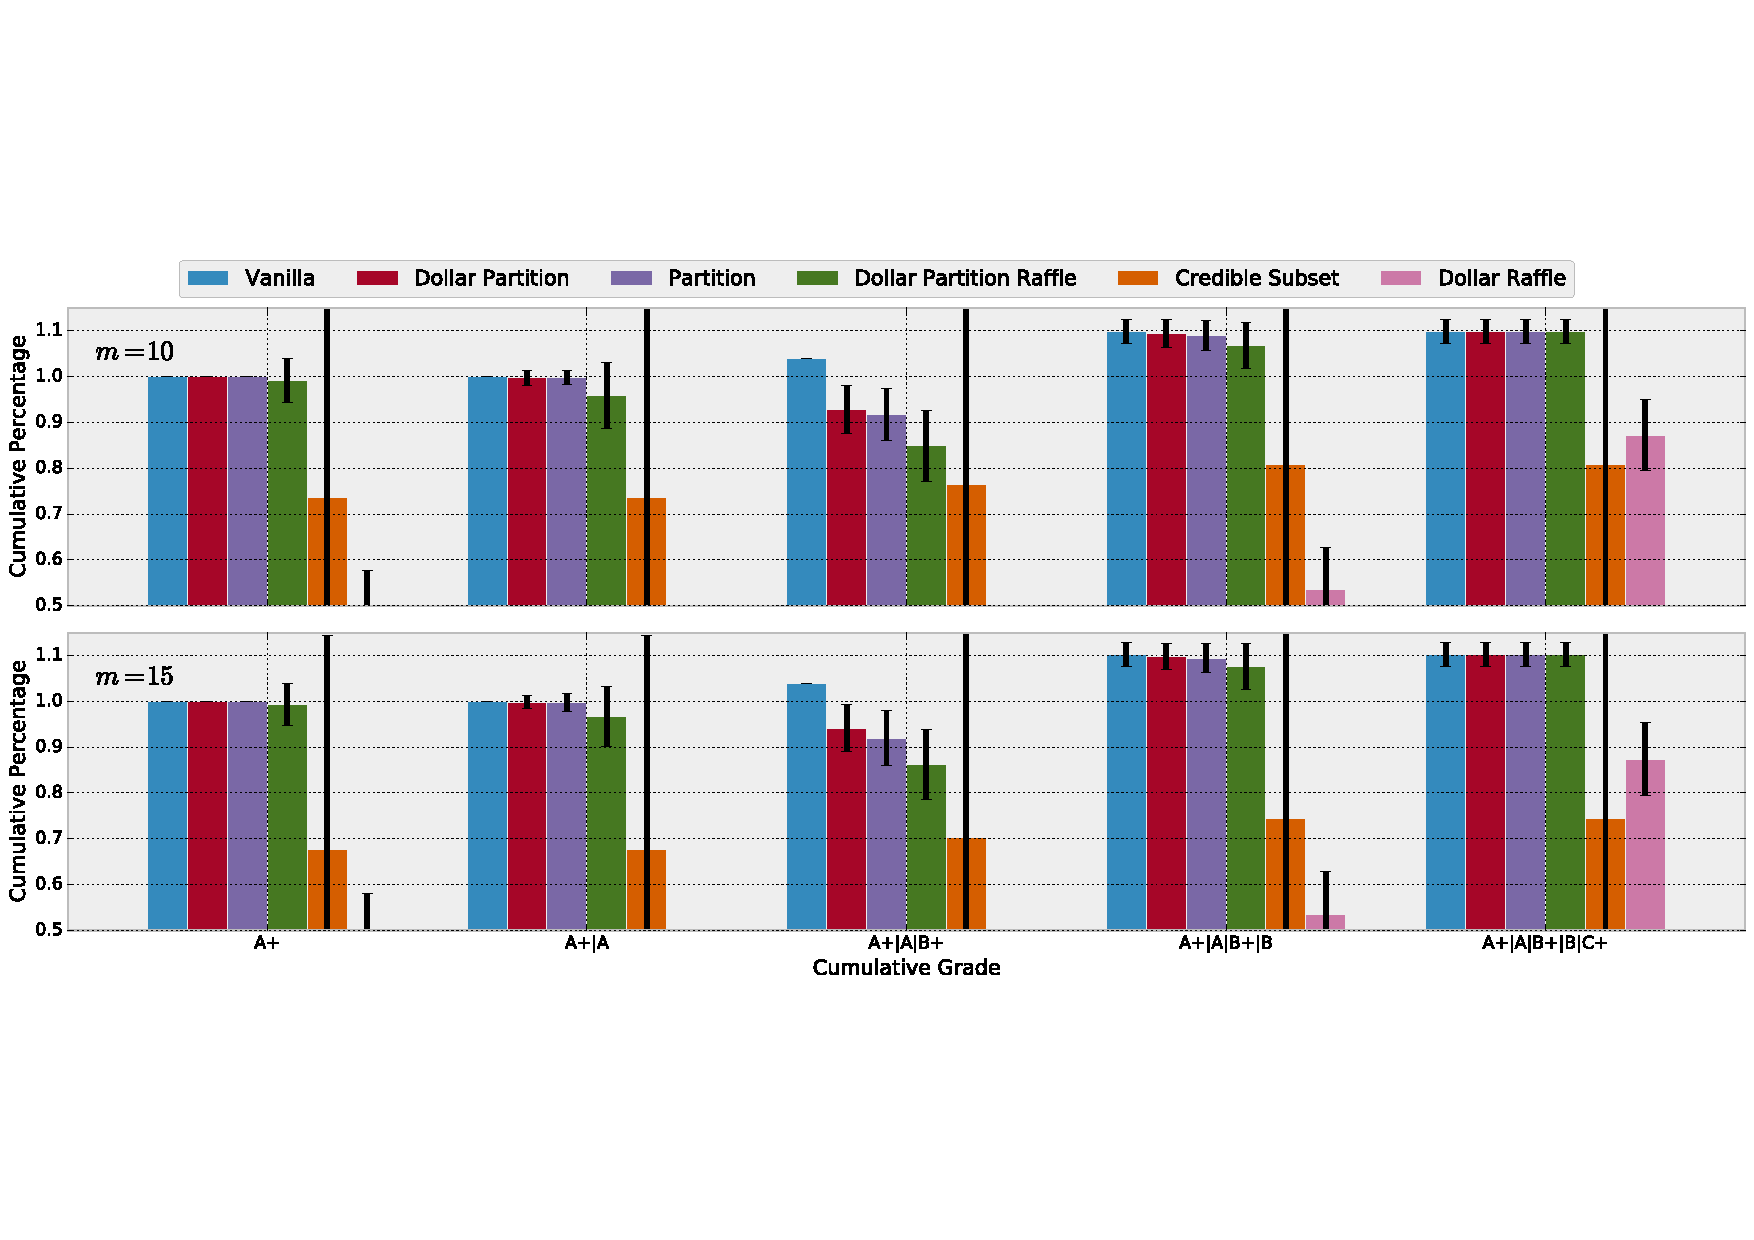
\includegraphics[width=.8\textwidth,height=1.8720000000000003in ]{./cumulative_grade_big-emb}
\caption{Mean cumulative percentage of each grade of agent selected by the six peer selection algorithms presented in this paper on 1000 random iterations selecting $k=25$ agents from a population of $n=130$ agents providing $m=10$ (top) and $m=15$ (bottom) reviews divided into $l=5$ clusters with a Mallows dispersion $\phi = 0.1$. To enable comparisons, every mechanism selects $|W|$ equal to that of Dollar Partition; hence the $\geq 1.0$ averages as $k=25$ is the denominator.
Error bars represent one standard deviation from the mean.
Dollar Partition selects more agents from a higher grade more often, selects more agents from a higher grade in the worst case, and does so more consistently, than any other strategyproof mechanism. To highlight Partition and Dollar Partition we have cropped results where they are the same (cutting off Dollar Raffle).}\label{fig:results}
\end{figure*}

Figure~\ref{fig:results} shows the performance of the six mechanisms discussed on two different metrics as we vary the number of reviews received. We fixed $\phi=0.1$ for this testing as setting $\phi \in \{0.0, 0.1, 0.25, 0.4\}$ had no significant effect. The graphs show the mean cumulative proportion of the agents in each grade that are selected by each of the mechanisms over 1000 samples. For instance, the 1.0 score received by Vanilla for both A+ and A+$|$A for all settings of $m$ mean that Vanilla always selects the 11 highest scoring agents in the ground truth ranking ($\sigma$). We use cumulative selection with respect to the ground truth ordering.  This partial sum is well defined for each set of grades and clearly shows where a particular mechanism is over- or under-performing. Each mechanism was allowed to select a number of proposals equal to the number of agents returned by Dollar Partition per iteration, hence the average cumulative selection is $>1.0$.
Whilst Vanilla is the best in our experiment, strictly dominating all other mechanisms, it is the only non-strategyproof mechanism. In practice, agents may not report truthfully with Vanilla and so it can perform much worse.
The other generalizations of Dollar are strictly dominated by Dollar Partition; our more nuanced mechanism yields a better selection.

Comparing Dollar Partition and Partition ($m=\{10,15\}$), both mechanisms select all of the A+ grade agents on every iteration.
Partition selects only $9/11$, in the worst case, of the A+$|$A, while Dollar Partition selects $10/11$, an $11\%$ improvement.
Considering the A+$|$A$|$B+ agents, Partition only selects $17/26$, while Dollar Partition selects $20/26$, a $\geq 17\%$ performance increase.
\vspace{-1.56mm}
\vspace{-3.15mm}
Neither mechanism ever selects an agent with rank lower than C+; even in the worst case, both perform better than every other strategyproof mechanism in our study.\footnote{It is hard to directly compare results for Credible Subset due to the large probability of returning an empty set. This problem is not easily overcome; removing the ability to return an empty set means Credible Subset is no longer strategyproof. When Credible Subset does return a set, it slightly outperforms other mechanisms.} Standard deviation is also higher for Partition for all these cases, indicating Partition is much more likely to make mistakes and select agents from a lower grade over agents in a higher grade. Dollar Partition performs better than Partition in the worst case, and performs better on average. In a low information setting (i.e., $m\leq5$), Partition does perform slightly better on average than Dollar Partition. However, Dollar Partition shows a lower variance and better worst case performance across all settings to $m$, demonstrating its robustness to lopsided clusterings.


\smallskip  \noindent
\textbf{General Results:} We explored a realistic part of the large parameter space to investigate the mechanisms. The practical upshot, after running hundreds of thousands of instances, is that there are numerous tradeoffs that system designers must consider, critically depending on their target domain. In general, varying other parameters, such as $k$, $\ell$, $D$ and $F$ did not change the ranking of mechanisms shown here. However, increasing the number of clusters improved Dollar Partition's performance in comparison to Partition's, which may stem from the increased chance that Partition will select the bottom candidates of a given cluster instead of better ranked candidates in a different cluster. Accordingly, as it generally selects the top candidates, Partition's performance improves when scoring rules are exponential in comparison to less extreme scoring rules, such as Borda.

Dollar Partition is much better when there is sufficient information, in terms of the number of reviews and the granularity of the grades, to have a chance of recovering the ground truth ordering. Settings like conferences with $n=2000$ papers and $m=5$ reviews split into 5--8 grades often have no clear cutoff between accept and reject; the grades contain too many items. In these cases all the mechanisms perform poorly, as selecting a set of winners is akin to randomly selecting agents from the set of possible winners. See, e.g., the NIPS experiment\footnote{http://blog.mrtz.org/2014/12/15/the-nips-experiment.html} and the recent paper on the limits of noisy rank aggregation using data from the KDD conference \cite{JoRa15a}. As the ratio of $m$ to $n$ grows, and the granularity of the grades increases, it becomes possible to recover the ground truth ranking, and Dollar Partition outperforms the other mechanisms.







\section{Conclusion}

We introduce a novel peer selection mechanism---Dollar Partition.
Overall, Dollar Partition's flexibility in setting the number of agents to be selected from each cluster addresses the worst-case instances where partitions may be lopsided, allowing Dollar Partition to reach higher quality, more consistent results than existing mechanisms. Combined with the ability to always return a winning set, it is an improvement over current mechanisms.  Among strategyproof mechanisms, Partition and Dollar Partition may
have a certain `psychological' advantage: they may incentivize agents to report truthfully because an agent's contribution in selecting other agents (with whom he is not competing) is more direct.
Moreover, partitioning into groups helps deal with conflict of interest cases, when there is fear of collusion among several agents; putting them in the same cluster prevents them from influencing one another's chance of success.
Peer selection is a fundamental problem that has received less attention than voting rules.  We envisage the need to develop robust solutions with good incentive properties, as these are widely applicable in large-scale, crowdsourcing settings.

\vspace{-0.86mm}
\vspace{-1.48mm}
\section*{Acknowledgments}
Data61 (formerly known as NICTA) is funded by the Australian Government through the Department of Communications and the Australian Research Council through the ICT Centre of Excellence Program. This research has also been partly funded by Microsoft Research through its PhD Scholarship Program, and by Israel Science Foundation grant \#1227/12. This work has also been partly supported by COST Action IC1205 on Computational Social Choice.

\normalsize
\bibliographystyle{aaai}  Aperiam hic odit architecto nisi cumque unde libero, quia suscipit eos quasi unde autem deleniti ea placeat quas ex voluptate, qui sed ex odit repellendus iste fuga voluptas ea laborum voluptates pariatur?\clearpage
\bibliography{abb,prizerefs}


\end{document}










